\documentclass[12pt,a4paper,fleqn]{ltjsarticle}

\usepackage{amsmath,amssymb}
\usepackage{setspace}
\usepackage{luatexja-ruby}
\usepackage{mathpazo}
\usepackage{graphicx}

\usepackage[OT1]{fontenc}

\setlength{\parindent}{1em}
\setlength{\mathindent}{2em}
\linespread{0.64}

\makeindex

\begin{document}

\title{世界で最も美しい数式}
\author{安田 健一}
\maketitle

\section{最終目的地}
以下に示す{\Large 「オイラーの式」}は、「世界で最も美しい数式」として知られているものである。
本文書の最終目的は、この数式の意味を理解することにある。
\begin{spacing}{0.3}
{\Large
    \begin{equation}
        e^{i\pi} + 1 = 0 \tag{$*$}
    \end{equation}
}
\end{spacing}

\section{定数の説明}
\begin{itemize}
    \item {\Large $e$:}
    自然対数の底

    ネイピア数とも呼ばれる。
    \begin{equation*}
        e = \lim_{x \to \infty} \left( 1 + \frac{1}{x} \right) ^x \notag
    \end{equation*}

    このような条件を満たす数として定義されている。
    このように$e$を定義すると、
    \begin{equation*}
        f(x) = e^x のとき、
        f'(x) = e^x
    \end{equation*}
    となる。
    具体的には、
    \begin{equation*}
        e = 2.7182818\dotsb
    \end{equation*}
    と続く無理数である。

    \item {\Large $i$:}
    虚数単位
    \begin{equation*}
        i = \sqrt{-1}
    \end{equation*}
    このような条件を満たす数として定義されている。

  \item {\Large $\pi$:}
    円周率

    円周の長さを、円の直径で割った数として定義されている。
    \begin{equation*}
        \pi = 3.141592\dotsb
    \end{equation*}
    と続く無理数である。
\end{itemize}

この式は$e, i, \pi, 1, 0$という全く独立に定められた、数学上極めて重要な定数が、
たった一つの式の中に見事に納められているため「世界で最も美しい数式」と呼ばれている。

\newpage

\section{オイラーの\ruby{公}{・}\ruby{式}{・}}
オイラーの式とは別に、オイラーの\ruby{公}{・}\ruby{式}{・}というものが存在する。
{\Large
    \begin{equation*}
        e^{i\theta} = \cos \theta + i\sin \theta \tag{$**$}
    \end{equation*}
}
これに、$\theta=\pi$ を代入すると、
\begin{align}
    e^{i\pi} &= \cos \pi + i\sin \pi \notag \\
             &= -1 + i \times 0 \qquad (\because \cos \pi = -1, \quad \sin \pi = 0) \notag \\
             &= -1 \notag
\end{align}

\begin{gather}
    e^{i\pi} = -1 \notag \\
    \therefore e^{i\pi} + 1 = 0 \qquad (オイラーの式) \notag
\end{gather}

このように、オイラーの式は、オイラーの\ruby{公}{・}\ruby{式}{・}の\textbf{特別な場合}であることが分かる。

\newpage

\section{オイラーの\ruby{公}{・}\ruby{式}{・}の証明}
\subsection{テイラー展開}
\begin{spacing}{0.3}
    \begin{align}
        f(x) &= \frac{f(0)}{0!}x^0+\frac{f'(0)}{1!}x^1+\frac{f''(0)}{2!}x^2
               +\frac{f'''(0)}{3!}x^3+\frac{f''''(0)}{4!}x^4+\frac{f'''''(0)}{5!}x^5+\dotsb \notag \\
             &= \sum_{n=0}^\infty \frac{f^{(n)}(0)}{n!}x^n \notag
    \end{align}
  関数$f(x)$を、このような\ruby{冪}{べき}級数($x^{n}$の和)に展開することを、「テイラー展開」という。

  (ここで$f^{(n)}(x)$は$f(x)$の$n$階微分、$n!$は$n$の階乗とする。)
\end{spacing}

\subsection{$e^x$のテイラー展開}
$e^x$をテイラー展開すると、次のようになることが知られている。
\begin{equation*}
    e^x = \frac{x^0}{0!}+\frac{x^1}{1!}+\frac{x^2}{2!}+\frac{x^3}{3!}
        + \frac{x^4}{4!}+\frac{x^5}{5!}+\frac{x^6}{6!}+\frac{x^7}{7!}+\dotsb
\end{equation*}

\subsection{三角関数のテイラー展開}
$\cos \theta$、$\sin \theta$を、テイラー展開すると、それぞれ次のようになることが知られている。
\begin{itemize}
    \item $\cos \theta$
        \begin{equation*}
            \cos \theta = \frac{\theta^0}{0!}-\frac{\theta^2}{2!}
                        + \frac{\theta^4}{4!}-\frac{\theta^6}{6!}+ \dotsb
        \end{equation*}

    \item $\sin \theta$
        \begin{equation*}
            \sin \theta = \frac{\theta^1}{1!}-\frac{\theta^3}{3!}
                        + \frac{\theta^5}{5!}-\frac{\theta^7}{7!}+ \dotsb
        \end{equation*}
\end{itemize}

\newpage

\subsection{$e^x$のテイラー展開の変形}
ここで、一つ大胆な発想をする。

この$e^x$のテイラー展開の式に$x=i\theta$を代入すると、
\begin{equation*}
    e^{i\theta} = \frac{\theta^0}{0!}+\frac{i\theta^1}{1!}-\frac{\theta^2}{2!}
                - \frac{i\theta^3}{3!}+\frac{\theta^4}{4!}+\frac{i\theta^5}{5!}
                - \frac{\theta^6}{6!}-\frac{i\theta^7}{7!}+ \dotsb
\end{equation*}
となる。
\begin{equation*}
    \because i^2 = -1
\end{equation*}

これを、$i$を含む項と、含まない項とで分別して整理すると、
\begin{equation*}
    e^{i\theta}= \underbrace{\left( \frac{\theta^0}{0!}-\frac{\theta^2}{2!}
                      + \frac{\theta^4}{4!}-\frac{\theta^6}{6!}+ \dotsb \right)}_{\cos \theta}
               +i\underbrace{\left( \frac{\theta^1}{1!}-\frac{\theta^3}{3!}
                      + \frac{\theta^5}{5!}-\frac{\theta^7}{7!}+ \dotsb \right)}_{\sin \theta}
\end{equation*}
と整理できる。

ここで、
\begin{align}
    \frac{\theta^0}{0!}-\frac{\theta^2}{2!}+\frac{\theta^4}{4!}-\frac{\theta^6}{6!}+ \dotsb &= \cos \theta \notag \\
    \frac{\theta^1}{1!}-\frac{\theta^3}{3!}+\frac{\theta^5}{5!}-\frac{\theta^7}{7!}+ \dotsb &= \sin \theta \notag
\end{align}
であるから、実数部分を$\cos \theta$、虚数部分を$\sin \theta$で書き直すと
\begin{equation*}
    e^{i\theta} = \cos \theta + i \sin \theta \tag{$**$}
\end{equation*}
となり、オイラーの\ruby{公}{・}\ruby{式}{・}が得られる。
\begin{flushright}
    Q.E.D
\end{flushright}

\section{オイラーの式の導出}
先に述べたとおり、オイラーの式は、オイラーの\ruby{公}{・}\ruby{式}{・}に$\theta=\pi$を代入することで
容易に導き出すことが出来る。
\begin{align}
    e^{i\pi} &= \cos \pi + i\sin \pi \notag \\
             &= -1 + i \times 0 \qquad (\because \cos \pi = -1, \quad \sin \pi = 0) \notag \\
             &= -1 \notag
\end{align}
{\LARGE
    \begin{equation*}
        \therefore e^{i\pi} + 1 = 0  \tag{$*$}
    \end{equation*}
}
を得ることになる。

\newpage

\section{幾何学的解釈}
\subsection{オイラーの\ruby{公}{・}\ruby{式}{・}の幾何学的解釈}
ここで$\cos\theta + i\sin\theta$ を複素平面上にプロットしてみると、

\begin{figure}[h]
  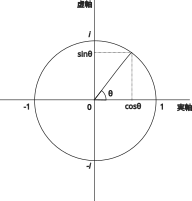
\includegraphics{circle.png}
    \caption{$e^{i\theta}=\cos\theta+i\sin\theta$の図}
\end{figure}

このように、$e^{i\theta}$は、
複素平面上で、動径$1$偏角$\theta$の、単位円上の一点に対応する。

\subsection{オイラーの式の幾何学的解釈}
\begin{figure}[h]
    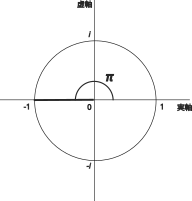
\includegraphics{circle-pi.png}
    \caption{$e^{i\pi}=-1$の図}
\end{figure}
このように、$e^{i\pi}=-1$は、
複素平面上で、動径$1$偏角$\pi(=180^{\circ})$の複素数は、実数$-1$に対応することを意味する。

要するに、オイラーの式は「複素平面上で、$180^\circ$回転させると$-1$(逆向き)になる。」
と解釈することが出来る。

\newpage

\section{オイラーの\ruby{公}{・}\ruby{式}{・}の周期性}
\begin{spacing}{0.3}
  \begin{align}
        e^{i(\theta+2\pi)} &= e^{i\theta}\cdot e^{2\pi} \notag \\
                           &= e^{i\theta}\cdot (\cos 2\pi + i\sin 2\pi) \notag \\
                           &= e^{i\theta}\cdot (1 + i \times 0) \notag \\
                           &= e^{i\theta} \notag
    \end{align}
    従って、$e^{i\theta}$は、$2\pi(=360^{\circ})$ 回転すると元に戻ることが分かる。
    これは、先の幾何学的な解釈ともきちんと一致する。
\end{spacing}

\section{終わりに}
ここまで見てきたように、オイラーの式は、単に数学的に重要な定数がきれいに詰め込まれているというだけでなく、
その解釈には、複素平面まで持ち出されるという非常に意味深いものであると言える。
このことが、この式が「世界で最も美しい数式」と呼ばれるゆえんである。

\vfill

\begin{flushright}
  Powered by \LaTeX
\end{flushright}

\end{document}
